%%%%%%%%%%%%%%%%%%%%%%%%%%%%%%%%%%%%%%%%%
% Beamer Presentation
% LaTeX Template
% Version 1.0 (10/11/12)
%
% This template has been downloaded from:
% http://www.LaTeXTemplates.com
%
% License:
% CC BY-NC-SA 3.0 (http://creativecommons.org/licenses/by-nc-sa/3.0/)
%
%%%%%%%%%%%%%%%%%%%%%%%%%%%%%%%%%%%%%%%%%

%----------------------------------------------------------------------------------------
%	PACKAGES AND THEMES
%----------------------------------------------------------------------------------------

\documentclass{beamer}

\mode<presentation> {

% The Beamer class comes with a number of default slide themes
% which change the colors and layouts of slides. Below this is a list
% of all the themes, uncomment each in turn to see what they look like.

%\usetheme{default}
%\usetheme{AnnArbor}
%\usetheme{Antibes}
%\usetheme{Bergen}
%\usetheme{Berkeley}
%\usetheme{Berlin}
%\usetheme{Boadilla}
%\usetheme{CambridgeUS}
%\usetheme{Copenhagen}
%\usetheme{Darmstadt}
%\usetheme{Dresden}
%\usetheme{Frankfurt}
%\usetheme{Goettingen}
%\usetheme{Hannover}
%\usetheme{Ilmenau}
%\usetheme{JuanLesPins}
%\usetheme{Luebeck}
\usetheme{Madrid}
%\usetheme{Malmoe}
%\usetheme{Marburg}
%\usetheme{Montpellier}
%\usetheme{PaloAlto}
%\usetheme{Pittsburgh}
%\usetheme{Rochester}
%\usetheme{Singapore}
%\usetheme{Szeged}
%\usetheme{Warsaw}

% As well as themes, the Beamer class has a number of color themes
% for any slide theme. Uncomment each of these in turn to see how it
% changes the colors of your current slide theme.

%\usecolortheme{albatross}
%\usecolortheme{beaver}
%\usecolortheme{beetle}
%\usecolortheme{crane}
%\usecolortheme{dolphin}
%\usecolortheme{dove}
%\usecolortheme{fly}
%\usecolortheme{lily}
%\usecolortheme{orchid}
%\usecolortheme{rose}
%\usecolortheme{seagull}
%\usecolortheme{seahorse}
%\usecolortheme{whale}
%\usecolortheme{wolverine}

%\setbeamertemplate{footline} % To remove the footer line in all slides uncomment this line
%\setbeamertemplate{footline}[page number] % To replace the footer line in all slides with a simple slide count uncomment this line

%\setbeamertemplate{navigation symbols}{} % To remove the navigation symbols from the bottom of all slides uncomment this line
}

\usepackage{graphicx} % Allows including images
\usepackage{booktabs} % Allows the use of \toprule, \midrule and \bottomrule in tables

%----------------------------------------------------------------------------------------
%	TITLE PAGE
%----------------------------------------------------------------------------------------

\title[Predictions in Financial Time Series]{Predictions in Financial Time Series} % The short title appears at the bottom of every slide, the full title is only on the title page

\author{Allan Steel} % Your name
\institute[ITB] % Your institution as it will appear on the bottom of every slide, may be shorthand to save space
{
Institute of Technology Blanchardstown \\ % Your institution for the title page
\medskip
\textit{allan@allansteel.com} % Your email address
}
\date{\today} % Date, can be changed to a custom date

\begin{document}

\begin{frame}
\titlepage % Print the title page as the first slide
\end{frame}

\begin{frame}
\frametitle{Contents} % Table of contents slide, comment this block out to remove it
\tableofcontents % Throughout your presentation, if you choose to use \section{} and \subsection{} commands, these will automatically be printed on this slide as an overview of your presentation
\end{frame}

%----------------------------------------------------------------------------------------
%	PRESENTATION SLIDES
%----------------------------------------------------------------------------------------

%------------------------------------------------
\section{Introduction} %
%------------------------------------------------

%\subsection{Subsection Example} % A subsection can be created just before a set of slides with a common theme to further break down your presentation into chunks

\begin{frame}
\frametitle{Introduction}
\begin{itemize}
\item Predicting Financial Time Series
\item Technical Analysis
\item Time Series Analysis
\end{itemize}

\end{frame}


%------------------------------------------------
\section{Data} %
%------------------------------------------------

\begin{frame}
\Huge{\centerline{Data}}
\end{frame}

% ---- Frame ------------
\begin{frame}
\frametitle{Data}
\begin{itemize}
\item Financial Data - time series
\item Yahoo
\item National Indices - geographical spread
\item UK, Germany, France, US, Japan, Australia
\end{itemize}
\end{frame}

% ---- Frame ------------
\begin{frame}
\frametitle{OHLC Data}
\begin{figure}
\centering
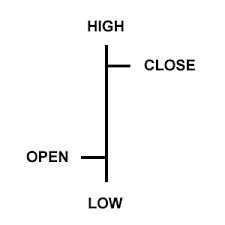
\includegraphics[width=6cm]{../Figures/chp3_ohlc}
\caption[]{A schematic representation of open, high, low and closing prices (OHLC)}
\label{fig:chp3_ohlc}
\end{figure}
\end{frame}

% ---- Frame ------------
\begin{frame}
\frametitle{German Dax}
% latex table generated in R 3.1.0 by xtable 1.7-3 package
% Wed May 28 17:41:24 2014
\begin{table}[ht]
\centering
\caption[Final 6 rows of the Dax data set.]{Final 6 rows of the Dax data set} 
\label{tab:daxtail}
\begin{tabular}{lcccc}
  \toprule Date & Open & High & Low & Close \\ 
  \midrule 13/12/2013 & 9017 & 9047 & 8991 & 9006 \\ 
  16/12/2013 & 9005 & 9188 & 8998 & 9164 \\ 
  17/12/2013 & 9143 & 9162 & 9085 & 9085 \\ 
  18/12/2013 & 9145 & 9191 & 9122 & 9182 \\ 
  19/12/2013 & 9280 & 9352 & 9257 & 9336 \\ 
  20/12/2013 & 9371 & 9413 & 9353 & 9400 \\ 
   \bottomrule \end{tabular}
\end{table}

\end{frame}

% ---- Frame ------------
%\begin{frame}
%\frametitle{German Dax Summary Statistics}
%\begin{table}[!htbp] \centering
%\caption[Dax summary statistics.]{Summary statistics of the Dax data set.}
%\label{tab:daxsum}
%\begin{tabular}{lccccc}
%\toprule
%Statistic & N & Mean & St. Dev & Min & Max \\
%\midrule
%Open  & 3,621 & 5,858.36 & 1,559.40 & 2,203.97 & 9,752.11 \\
%High  & 3,621 & 5,906.70 & 1,561.17 & 2,319.65 & 9,794.05 \\
%Low   & 3,621 & 5,804.85 & 1,557.49 & 2,188.75 & 9,714.02 \\
%Close & 3,621 & 5,857.74 & 1,559.39 & 2,202.96 & 9,742.96 \\
%\bottomrule
%%\normalsize
%\end{tabular}
%\end{table}
%\end{frame}

% ---- Frame ------------
\begin{frame}
\frametitle{German Dax 2000 to 2013}
\begin{figure}
\centering
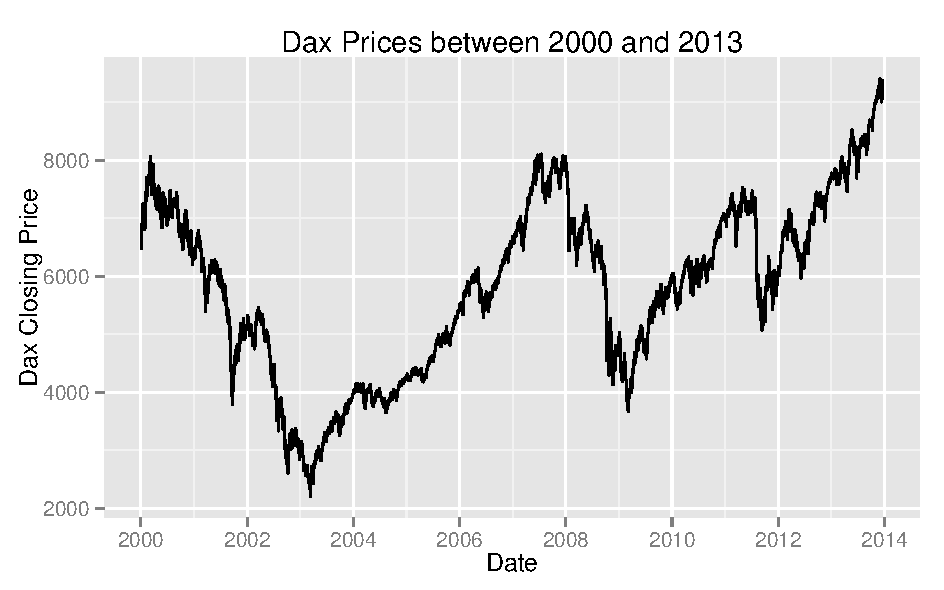
\includegraphics[width=10cm]{../Figures/chp3_dax_2000_2013}
\caption{Graph of German Dax in 2013.}
\label{fig:chp3_dax_2000_2013}
\end{figure}

\end{frame}

%------------------------------------------------
\section{Technical Analysis} %
%------------------------------------------------

\begin{frame}
\Huge{\centerline{Technical Analysis}}
\end{frame}

% ---- Frame ------------
\begin{frame}
\frametitle{Technical Analysis}
\begin{itemize}
\item Technical analysis is the study of historical prices \pause
\item Practitioners of technical analysis in the past were referred to as chartists \pause
\item All that was needed to know about a particular market was contained in its pricing chart
\end{itemize}

\end{frame}

% ---- Frame ------------
\begin{frame}
\frametitle{Technical Analysis}

\textit{\textquotedblleft Obviously I am biased against the chartist. This is not only a personal predilection, but a professional one as well. Technical Analysis is anathema to the academic world. We love to pick on it. Our bullying tactics are prompted by two considerations: (1) the method is patently false; and (2) it's easy to pick on. And while it may seem a bit unfair to pick on such a sorry target, just remember: it is your money we are trying to save.\textquotedblright}
%\footnotesize{
\begin{thebibliography}{99} % Beamer does not support BibTeX so references must be inserted manually as below
\bibitem[Malkiel, 1999]{p1} Malkiel, B.G. (1999)
\newblock A Random Walk Down Wall Street: Including a Life-cycle Guide to Personal Investing
\end{thebibliography}

\end{frame}

% ---- Frame ------------
\begin{frame}
\frametitle{Technical Indicators}

\begin{itemize}
\item Moving Average Convergence Divergence (MACD) \pause
\item Aroon \pause
\item Stochastic \pause
\item Rate of Change (ROC) \pause
\item Candlesticks 
\end{itemize}

\end{frame}

% ---- Frame ------------
\begin{frame}
\frametitle{Moving Average Convergence Divergence (MACD)}

MACD is a widely used technical indicator which attempts to detect the early stage of a market trend. Subtract a long exponential moving average (EMA) from a shorter one. The EMA is calculated as follows:

\[ EMA(n)_{t} = \dfrac{2}{n+1}(P_{t}-EMA_{t-1}) + EMA_{t-1}\]

Where $ P_{t} $ is the closing price of a market on day $ t $ and $ n $ is the number of periods used in calculating the moving average. MACD itself is calculated as:

\[ MACD_{t} = EMA(s)_{t} - EMA(l)_{t} \]

where $ EMA(s)_{t} $ is the short moving average and $ EMA(l)_{t} $ is the long one. In addition an EMA of the MACD itself is calculated in order to generate trade signals and is often referred to as the \textquotedblleft trigger line".

\end{frame}

% ---- Frame ------------
\begin{frame}
\frametitle{Moving Average Convergence Divergence (MACD)}

\begin{figure}
\centering
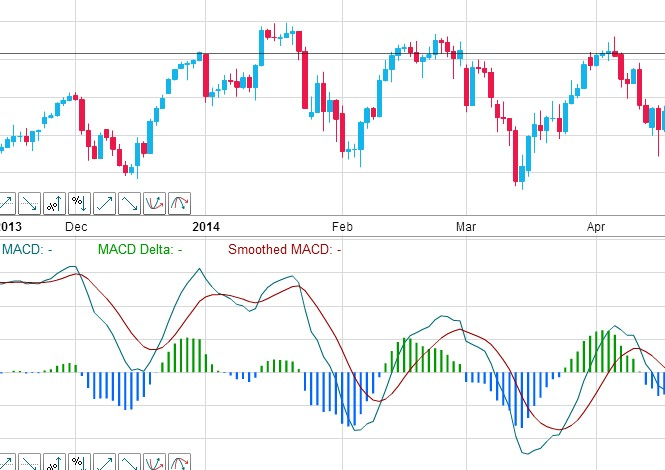
\includegraphics[width=8cm]{../Figures/presentation_macd}
\caption{Graph of Financial Data with MACD Added.}
\label{fig:presentation_macd}
\end{figure}


\end{frame}

%------------------------------------------------
\section{Time Series Analysis} %
%------------------------------------------------

\begin{frame}
\Huge{\centerline{Time Series}}
\end{frame}

% ---- Frame ------------
\begin{frame}
\frametitle{Time Series}

\begin{itemize}
\item ARIMA
\item Hybrid ARIMA
\end{itemize}

\end{frame}

% ---- Frame ------------
\begin{frame}
\frametitle{ARIMA}

\begin{itemize}
\item Plot the data to get a general feel for the time series and to establish if it is stationary.  \pause
\item Stabilize any variance in the data with a transformation process such as the Box-Cox method. \pause
\item Arima models work with stationary data, so if necessary, take differences of the data until it is stationary. \pause
\item Examine the auto-correlation and partial auto-correlation (ACF/PACF) plots in order to determine if an AR(p) or MA(q) model is appropriate. \pause
\item Test the chosen model(s), using the AICc to determine if a better model is available. \pause
\item Check the residuals from the best model by plotting the ACF, and doing a portmanteau test on them. If the results from these tests do not look like white noise, a modified model may be required. \pause
\item Finally, once the residuals have a similar pattern to white noise, the model can be used to generate forecasts.   
\end{itemize}

\end{frame}

% ---- Frame ------------
\begin{frame}
\frametitle{Hybrid ARIMA Models}
\begin{figure}
\centering
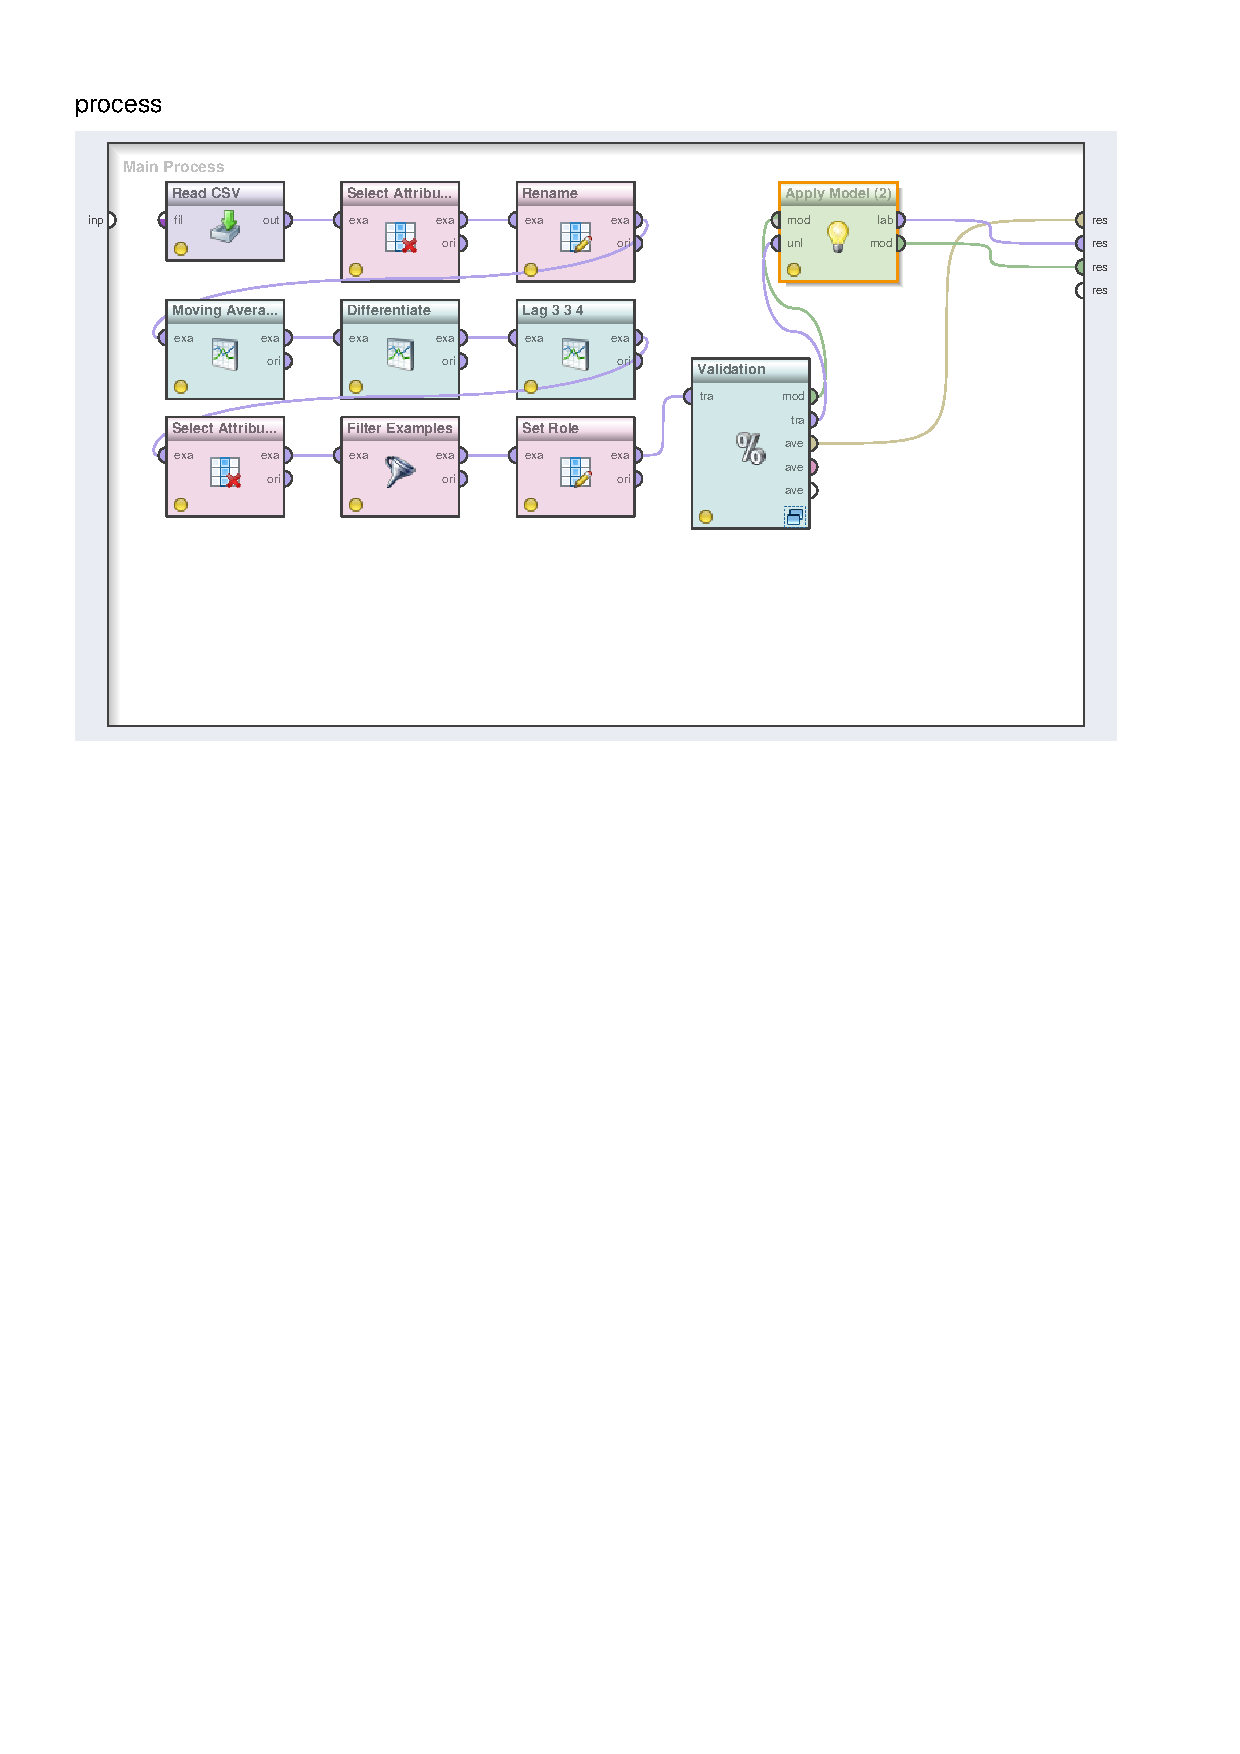
\includegraphics[width=10cm]{../Figures/chp_ts_rm_arima}
\caption{Rapid Miner Hybrid ARIMA Model}
\label{fig:chp_ts_rm_arima}
\end{figure}



\end{frame}

%------------------------------------------------
\section{Results} %
%------------------------------------------------

\begin{frame}
\Huge{\centerline{Results}}
\end{frame}

% ---- Frame ------------
\begin{frame}
\frametitle{Results}

\begin{itemize}
\item Baseline Systems - for comparisons.
	\begin{itemize}
	\item Buy and Hold
	\item Reversing System
	\end{itemize}
\item Technical Analysis
	\begin{itemize}
	\item Trend Detection Indicators
	\item Reversal Indicators
	\item Momentum Indicators
	\item Break-out Systems
	\item Candlesticks
	\end{itemize}
\item ARIMA and Hybrid ARIMA
	\begin{itemize}
	\item Predicting closing price
	\item Predicting Up or Down
	\end{itemize}
\end{itemize}

\end{frame}

% ---- Frame ------------
\begin{frame}
\Huge{\centerline{Buy and Hold}}
\Huge{\centerline{Reversing System}}
\end{frame}

% ---- Frame ------------
\begin{frame}
\frametitle{Results - Baseline Buy and Hold}

% latex table generated in R 3.1.0 by xtable 1.7-3 package
% Tue Aug 19 13:19:47 2014
\begin{table}[ht]
\centering
\caption[Results from the Naive Long System trading close to close]{Naive Long System changed such that the trading period is the previous close price minus today's close.} 
\label{tab:nlng_results_2}
\begin{tabular}{lccc}
  \toprule Mkt & LongPL & L Win \% & Av L PL \\ 
  \midrule DAX & 2649 & 53 & 1 \\ 
  CAC & -1667 & 51 & 0 \\ 
  FTSE & 86 & 51 & 0 \\ 
  Dow & 5219 & 53 & 1 \\ 
  Nikkei & -2712 & 51 & -1 \\ 
  AORD & 2229 & 53 & 1 \\ 
   \bottomrule \end{tabular}
\end{table}


\end{frame}

% ---- Frame ------------
\begin{frame}
\frametitle{Results - Baseline Daily Reversal}

% latex table generated in R 3.1.0 by xtable 1.7-3 package
% Mon Jun 02 13:01:39 2014
\begin{table}[ht]
\centering
\caption[Naive Following System.]{Naive system which repeats the previous day's trade direction.} 
\label{tab:ntfresults}
\begin{tabular}{lcccccc}
  \toprule Mkt & LongPL & ShortPL & L Win \% & L Trades & S Win \% & S Trades \\ 
  \midrule Dax & -3131 & -947 & 51 & 1826 & 47 & 1672 \\ 
  CAC & -7810 & -940 & 47 & 1786 & 47 & 1798 \\ 
  F100 & -4115 & -4284 & 50 & 1815 & 47 & 1712 \\ 
  Dow & -6047 & -15799 & 51 & 1870 & 44 & 1646 \\ 
  Nik & -20486 & -2324 & 46 & 1665 & 49 & 1769 \\ 
  Oz & -237 & -1264 & 52 & 1851 & 47 & 1682 \\ 
   \bottomrule \end{tabular}
\end{table}


\end{frame}

% ---- Frame ------------
\begin{frame}
\Huge{\centerline{Technical Analysis}}
\Huge{\centerline{ }}
\Huge{\centerline{Aroon}}
\Huge{\centerline{Break-out System}}
\end{frame}

% ---- Frame ------------
\begin{frame}
\frametitle{Results - Aroon Technical Indicator}

% latex table generated in R 3.1.0 by xtable 1.7-3 package
% Mon Aug 11 19:25:43 2014
\begin{table}[ht]
\centering
\caption[Results from a system based on the Aroon indicator]{Results from a system based on the Aroon indicator.} 
\label{tab:aroon_results}
\begin{tabular}{lcccccc}
  \toprule Mkt & LongPL & ShortPL & L Win \% & Av L PL & S Win \% & Av S PL \\ 
  \midrule DAX & 5308 & 5257 & 56 & 3 & 51 & 4 \\ 
  CAC & -1638 & 4919 & 50 & -1 & 52 & 4 \\ 
  FTSE & 3042 & 5715 & 52 & 2 & 51 & 5 \\ 
  Dow & 12131 & 3811 & 55 & 7 & 49 & 3 \\ 
  Nikkei & -4852 & 12013 & 49 & -3 & 52 & 10 \\ 
  AORD & 3735 & 3540 & 55 & 2 & 50 & 3 \\ 
   \bottomrule \end{tabular}
\end{table}


\end{frame}

% ---- Frame ------------
\begin{frame}
\frametitle{Results - Break-out Indicator}

% latex table generated in R 3.1.0 by xtable 1.7-3 package
% Tue Aug 12 20:06:52 2014
\begin{table}[ht]
\centering
\caption[Results from the Daily High/Low Breakout System]{Results from the Daily High/Low Breakout System.} 
\label{tab:hl_bout_sys}
\begin{tabular}{lcccccc}
  \toprule Mkt & LongPL & ShortPL & L Win \% & Av L PL & S Win \% & Av S PL \\ 
  \midrule DAX & 12225 & 13411 & 55 & 7 & 54 & 8 \\ 
  CAC & 3491 & 6955 & 53 & 2 & 53 & 4 \\ 
  FTSE & 13189 & 18481 & 59 & 7 & 59 & 12 \\ 
  Dow & -19598 & -28337 & 42 & -11 & 38 & -17 \\ 
  Nikkei & 31988 & 43554 & 57 & 19 & 58 & 27 \\ 
  AORD & 17225 & 19184 & 66 & 10 & 65 & 13 \\ 
   \bottomrule \end{tabular}
\end{table}

\end{frame}

% ---- Frame ------------
\begin{frame}
\frametitle{Results - Break out compared to Reversing System}

% latex table generated in R 3.1.0 by xtable 1.7-3 package
% Tue Jun 10 16:51:55 2014
\begin{table}[ht]
\centering
\caption[Daily High / Low Breakout System compared with Naive Reversing System]{Results from Daily High / Low Breakout System compared with Naive Reversing System} 
\label{ab:hl_bout_sys_diff}
\begin{tabular}{lcccccc}
  \toprule Mkt & LongPL & ShortPL & L Win \% & Av L PL & S Win \% & Av S PL \\ 
  \midrule Dax & 20126 & 18098 & 5 & 10 & 7 & 11 \\ 
  CAC & 13312 & 12366 & 5 & 7 & 6 & 8 \\ 
  FTSE & 8955 & 14499 & 6 & 4 & 9 & 10 \\ 
  Dow & -35154 & -33381 & -14 & -21 & -11 & -20 \\ 
  Nikkei & 72276 & 61159 & 13 & 43 & 10 & 37 \\ 
  AORD & 18083 & 21007 & 14 & 10 & 17 & 14 \\ 
   \bottomrule \end{tabular}
\end{table}

\end{frame}

% ---- Frame ------------
\begin{frame}
\Huge{\centerline{Hybrid ARIMA Models}}
\Huge{\centerline{ }}
\Huge{\centerline{Predicting Closing Price}}
\Huge{\centerline{Predicting Up or Down}}
\end{frame}

% ---- Frame ------------
\begin{frame}
\frametitle{Results - Predicting closing Price with ARIMA}

% latex table generated in R 3.1.0 by xtable 1.7-3 package
% Sun Jun 29 08:18:19 2014
\begin{table}[ht]
\centering
\caption[Forecasts generated by the ARIMA models used in the System 1 algorithm]{Forecasts generated by the ARIMA models used in the System 1 algorithm.} 
\label{tab:chp_ts:arima1}
\begin{tabular}{lcccccc}
  \toprule Mkt & LongPL & ShortPL & L Win \% & Av L PL & S Win \% & Av S PL \\ 
  \midrule Dax & -644 & -1881 & 50 & -3 & 41 & -7 \\ 
  CAC & 1555 & 850 & 59 & 6 & 51 & 3 \\ 
  FTSE & 531 & -708 & 53 & 2 & 46 & -2 \\ 
  Dow & 3130 & -1766 & 58 & 14 & 48 & -6 \\ 
  Nikkei & 41 & -1157 & 48 & 0 & 45 & -5 \\ 
  AORD & 679 & -204 & 55 & 3 & 49 & -1 \\ 
   \bottomrule \end{tabular}
\end{table}


\end{frame}

% ---- Frame ------------
\begin{frame}
\frametitle{Results - Predicting closing Price with Hybrid ARIMA/k-NN}

%% latex table generated in R 3.1.0 by xtable 1.7-3 package
% Sun Jun 29 08:18:31 2014
\begin{table}[ht]
\centering
\caption[Results from passing closing price predictions from hybrid ARIMA/k-NN model to System 1]{Results from passing closing price predictions from hybrid ARIMA/k-NN model to System 1.} 
\label{tab:chp_ts:pred_close_arima_knn_sys1}
\begin{tabular}{lcccccc}
  \toprule Mkt & LongPL & ShortPL & L Win \% & Av L PL & S Win \% & Av S PL \\ 
  \midrule Dax & 8270 & 9900 & 56 & 4 & 52 & 6 \\ 
  CAC & 6284 & 12597 & 54 & 3 & 55 & 7 \\ 
  FTSE & 17605 & 17026 & 58 & 9 & 56 & 10 \\ 
  Dow & 30330 & 20549 & 59 & 17 & 53 & 12 \\ 
  Nikkei & 15374 & 33366 & 54 & 9 & 57 & 20 \\ 
  AORD & 7658 & 6638 & 57 & 4 & 53 & 4 \\ 
   \bottomrule \end{tabular}
\end{table}

% latex table generated in R 3.1.0 by xtable 1.7-3 package
% Sat Aug 16 11:48:15 2014
\begin{table}[ht]
\centering
\caption[Mean PL from hybrid ARIMA/k-NN models minus mean PL from Naive Reverse system]{Results from a system using forecasts from a ARIMA/k-NN model with the results of the Naive Reversing System subtracted.} 
\label{tab:chp_ts:pred_close_arima_knn_sys1_diff}
\begin{tabular}{lcccc}
  \toprule Mkt & L Win \% & Av L PL & S Win \% & Av S PL \\ 
  \midrule DAX & -1 & -1 & -4 & -2 \\ 
  CAC & -1 & -2 & -3 & -3 \\ 
  FTSE & 1 & -2 & 0 & -3 \\ 
  Dow & 1 & 1 & -3 & -7 \\ 
  Nikkei & -3 & -1 & -4 & -10 \\ 
  AORD & 0 & 0 & 2 & 7 \\ 
   \bottomrule \end{tabular}
\end{table}


\end{frame}

% ---- Frame ------------
\begin{frame}
\frametitle{Results - Predicting Up/Down Categorical Label with Hybrid ARIMA/k-NN }

%% latex table generated in R 3.1.0 by xtable 1.7-3 package
% Tue Jul 22 20:47:45 2014
\begin{table}[ht]
\centering
\caption[Results from a trading system using the forecast of categorical label "U/D" from hybrid ARIMA/k-NN model]{Results from a trading system using the forecast of categorical label "U/D" from hybrid ARIMA/k-NN model.} 
\label{tab:chp_ts:pUD_CAT_arima_knn_sys}
\begin{tabular}{lcccccc}
  \toprule Mkt & LongPL & ShortPL & L Win \% & Av L PL & S Win \% & Av S PL \\ 
  \midrule Dax & 15692 & 17357 & 61 & 8 & 60 & 12 \\ 
  CAC & 10161 & 16587 & 60 & 6 & 59 & 9 \\ 
  FTSE & 15553 & 14960 & 60 & 8 & 60 & 10 \\ 
  Dow & 30347 & 20624 & 62 & 14 & 60 & 15 \\ 
  Nikkei & 27206 & 45031 & 60 & 18 & 60 & 24 \\ 
  AORD & 9711 & 8751 & 60 & 5 & 59 & 6 \\ 
   \bottomrule \end{tabular}
\end{table}

% latex table generated in R 3.1.0 by xtable 1.7-3 package
% Tue Jul 22 20:47:45 2014
\begin{table}[ht]
\centering
\caption[Predicting UpDn CAT - Arima/k-NN predictions passed to System 4 - ]{Results from Naive Reversing System subtracted from results generated from predicting Up/Down categorical label using Arima/k-NN.} 
\label{tab:chp_ts:pUD_CAT_arima_knn_sys_diff}
\begin{tabular}{lcccccc}
  \toprule Mkt & LongPL & ShortPL & L Win \% & Av L PL & S Win \% & Av S PL \\ 
  \midrule Dax & 14745 & 14226 & 8 & 7 & 11 & 10 \\ 
  CAC & 9221 & 8777 & 7 & 5 & 6 & 5 \\ 
  FTSE & 11269 & 10845 & 7 & 5 & 10 & 8 \\ 
  Dow & 14548 & 14577 & 6 & 4 & 11 & 12 \\ 
  Nikkei & 24882 & 24545 & 9 & 17 & 6 & 12 \\ 
  AORD & 8447 & 8514 & 7 & 4 & 11 & 6 \\ 
   \bottomrule \end{tabular}
\end{table}


\end{frame}

% ---- Frame ------------
\begin{frame}
\frametitle{Results - Predicting Up/Down Numerical Label Hybrid ARIMA/k-NN}

%% latex table generated in R 3.1.0 by xtable 1.7-3 package
% Sun Jun 29 08:18:37 2014
\begin{table}[ht]
\centering
\caption[Results from a trading system using the forecast of a continous label from a hybrid ARIMA/ANN model]{Results from a trading system using the forecast of a continous label from a hybrid ARIMA/k-NN model.} 
\label{tab:chp_ts:pUD_01_arima_knn_sys}
\begin{tabular}{lcccccc}
  \toprule Mkt & LongPL & ShortPL & L Win \% & Av L PL & S Win \% & Av S PL \\ 
  \midrule Dax & 14122 & 15787 & 64 & 11 & 55 & 7 \\ 
  CAC & 11115 & 17540 & 65 & 10 & 57 & 7 \\ 
  FTSE & 18156 & 17563 & 65 & 14 & 56 & 8 \\ 
  Dow & 28106 & 18383 & 66 & 20 & 55 & 9 \\ 
  Nikkei & 21724 & 39549 & 63 & 25 & 57 & 15 \\ 
  AORD & 9607 & 8647 & 65 & 7 & 56 & 4 \\ 
   \bottomrule \end{tabular}
\end{table}

% latex table generated in R 3.1.0 by xtable 1.7-3 package
% Mon Jul 07 19:18:18 2014
\begin{table}[ht]
\centering
\caption[Predicting UpDn 01 - Arima/k-NN predictions passed to System 3.]{Results from Naive Reversing System subtracted from results generated from predicting Up/Down Numerical label using Arima/k-NN.} 
\label{tab:chp_ts:pUD_01_arima_knn_sys_diff}
\begin{tabular}{lcccccc}
  \toprule Mkt & LongPL & ShortPL & L Win \% & Av L PL & S Win \% & Av S PL \\ 
  \midrule Dax & 13175 & 12656 & 11 & 10 & 6 & 5 \\ 
  CAC & 10175 & 9730 & 12 & 9 & 4 & 3 \\ 
  FTSE & 13872 & 13448 & 12 & 11 & 6 & 6 \\ 
  Dow & 12307 & 12336 & 10 & 10 & 6 & 6 \\ 
  Nikkei & 19400 & 19063 & 12 & 24 & 3 & 3 \\ 
  AORD & 8343 & 8410 & 12 & 6 & 8 & 4 \\ 
   \bottomrule \end{tabular}
\end{table}


\end{frame}


%------------------------------------------------
\section{Conclusions} %
%------------------------------------------------
% ---- Frame ------------
\begin{frame}
\frametitle{Conclusions}

\begin{itemize}
\item Technical Analysis Indicators - generally not good \pause
\item Break-out system - very good \pause
\item ARIMA - not good \pause
\item Hybrid ARIMA models - good with k-NN
\end{itemize}

\end{frame}

%------------------------------------------------

\begin{frame}
\Huge{\centerline{The End}}
\end{frame}

%----------------------------------------------------------------------------------------

\end{document} 